 \begin{frame}{Summary}
    \emph{Use the perception of a smart environment and its agents to recognize the conversational state and expectations of inhabitants towards different kinds of artificial agents.}
    \centering\\
    \vspace{10pt}
    \resizebox{1.\textwidth}{!}{%
        \footnotesize
        \begin{tikzpicture}
        \action<2->{\node (a) at (0,0)
        {
          \resizebox{.25\textwidth}{!}{%
            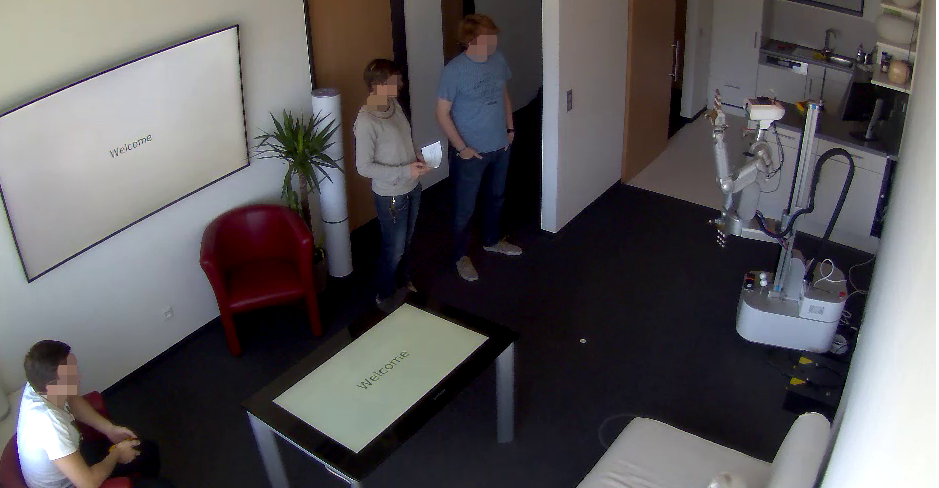
\includegraphics[trim={8cm 0 2cm 0},clip]{study-addressee-vp57}
          }
        };}
        \action<2->{\node[align=left, anchor=north, text width=.25\textwidth] (at) at (0, -.11\textwidth) {
        \textbf{RQ1 \scriptsize Addressing Behaviour}\\
          \vspace{5pt}
          \textcolor{mygreen}{\faCheckCircle} \Naive{} addressing\\
          \textcolor{mygreen}{\faCheckCircle} Attention\\
          \textcolor{mygreen}{\faCheckCircle} Speech
          };}
        \action<3->{\node (b) at (.25\textwidth+10,0)
        {
          \resizebox{.25\textwidth}{!}{%
            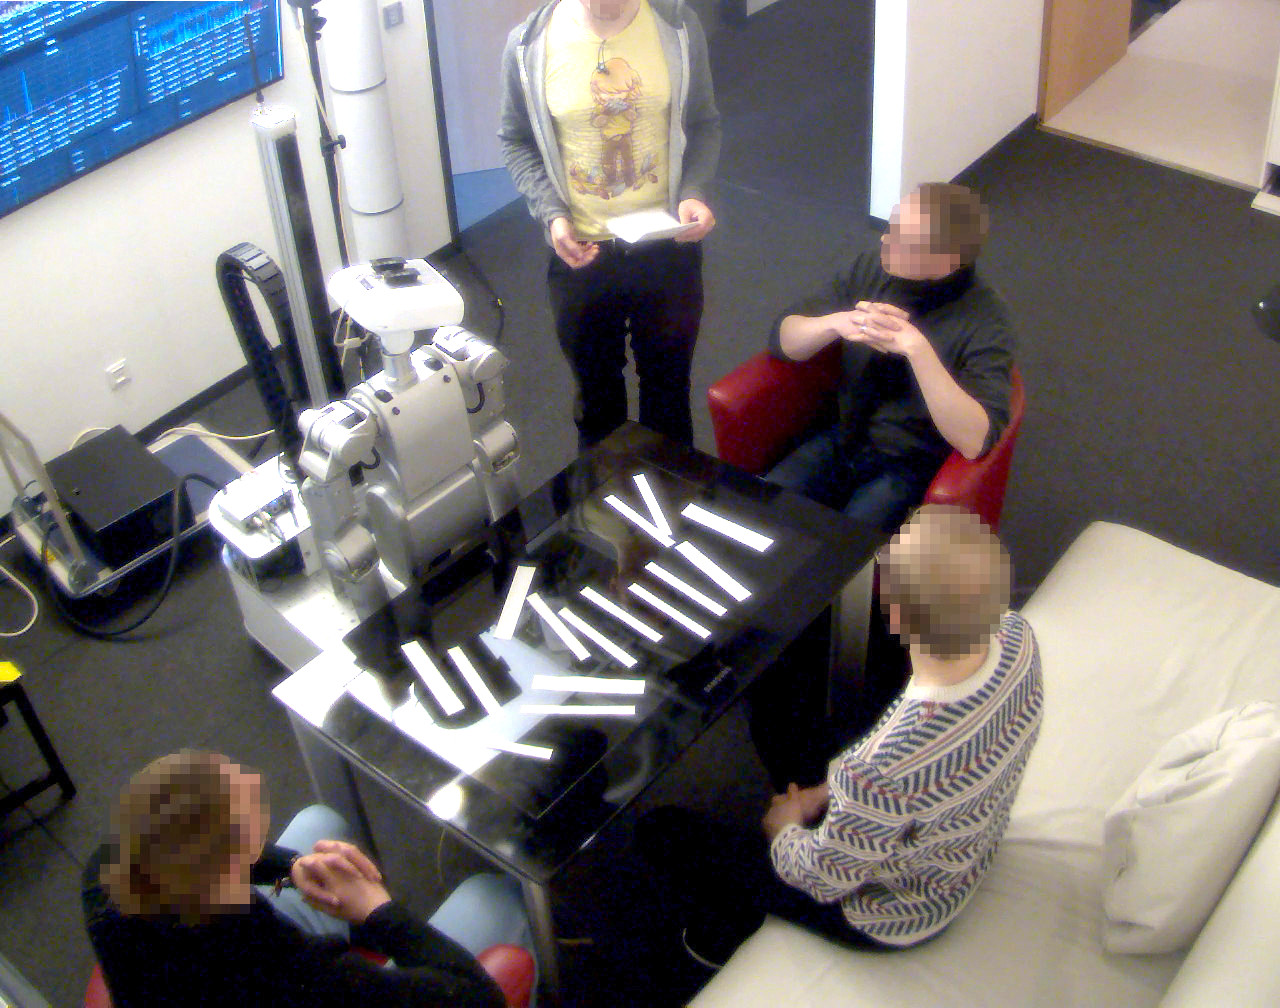
\includegraphics[trim={0 0 0 2cm},clip]{addressee-meka-intro}
          }
        };}
        \action<3->{\node[align=left, anchor=north, text width=.25\textwidth] (bt) at (.25\textwidth+10, -.11\textwidth) {
          \textbf{RQ2 \scriptsize Addressee Recognition}\\
          \vspace{5pt}
          \textcolor{mygreen}{\faCheckCircle} Mouth movements\\
          \textcolor{mygreen}{\faCheckCircle} Mutual gaze\\
          \textcolor{mygreen}{\faCheckCircle} Addressee\\
          };}
        \action<4->{\node (c) at (.5\textwidth+20,0)
        {
          \resizebox{.25\textwidth}{!}{%
            \input{generated/conversational_group_defence.pdf_tex}
          }
        };}
        \action<4->{\node[align=left, anchor=north, text width=.25\textwidth] (ct) at (.5\textwidth+20, -.11\textwidth) {
          \textbf{RQ3 \scriptsize Conversational Group}\\
          \vspace{5pt}
          \textcolor{mygreen}{\faCheckCircle} F-Formation\\
          \textcolor{mygreen}{\faCheckCircle} Ga\-ze di\-rec\-tion\\
          \textcolor{mygreen}{\faCheckCircle} Face detection\\
          };}
        \action<5->{\node (d) at (.75\textwidth+30,0)
        {
          \resizebox{.25\textwidth}{!}{%
            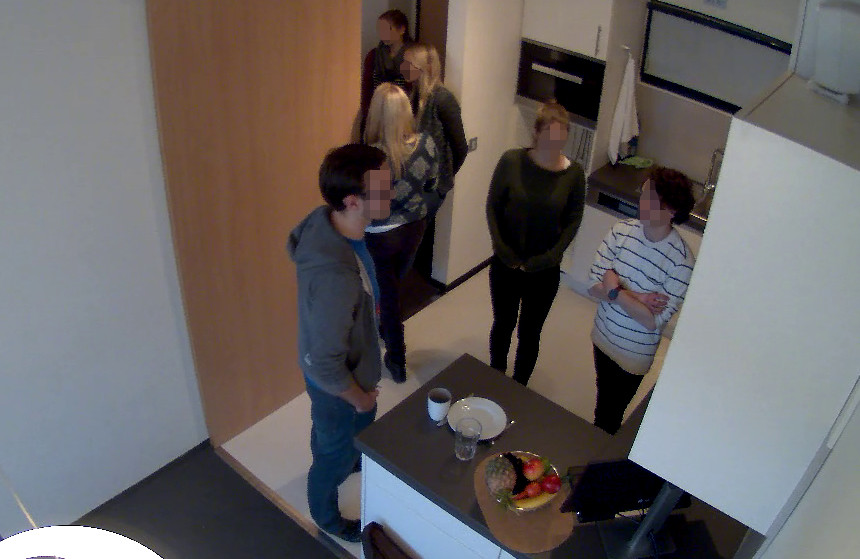
\includegraphics[trim={4.1cm 0 0 0},clip]{conversational_group}
          }
        };}
        \action<5->{\node[align=left, anchor=north, text width=.25\textwidth] (dt) at (.75\textwidth+30, -.11\textwidth) {
          \textbf{RQ4 \scriptsize Conversational Roles}\\
          \vspace{5pt}
          \textcolor{mygreen}{\faCheckCircle} Simple Models\\
          \textcolor{myred}{\faTimesCircle} Low-Level Features\\
          \textcolor{mygreen}{\faCheckCircle} Time Sequences\\
        };}
\end{tikzpicture}
      }
  \pnote{3}
\end{frame}
\subsection{Outlook}
\begin{frame}{Interaction in Smart Environments - Outlook}
  \begin{columns}[T] % align columns
    \begin{column}{.65\textwidth}
    \centering
    \resizebox{1.\textwidth}{!}{%
        \footnotesize
        \begin{tikzpicture}
        \action<1->{\node (a) at (0,0)
        {
          \resizebox{\textwidth}{!}{%
            
\includegraphics[width=\textwidth]{generated/csra-shots.pdf}
          }
        };}
      \end{tikzpicture}
    }
    \end{column}%
    \begin{column}{.4\textwidth}
      \footnotesize
          \textbf{Future Work}\\
          \vspace{5pt}
          {\onslide<2->{\textcolor{mygreen}{\faSearchPlus} Input Models (Face, Gaze, Person)\\}}
          {\onslide<3->{\textcolor{mygreen}{\faSearchPlus} Group Detection Edge Cases\\}}
          {\onslide<4->{\textcolor{mygreen}{\faSearchPlus} Amount of Data\\}}
          \vspace{10pt}
          \onslide<5->{\textbf{Applications}}\\
          \vspace{5pt}
          {\onslide<6->{\textcolor{mygreen}{\faThumbsUp} Addressee: Enhance Interaction\\}}
          {\onslide<7->{\textcolor{mygreen}{\faThumbsUp} Group: Analyse Dynamics, Properties\\}}
          {\onslide<8->{\textcolor{mygreen}{\faThumbsUp} Role: Adapt Behaviour, Repair Communication\\}}
    \end{column}%
    \end{columns}
  \pnote{0}
\end{frame}
 \begin{frame}[standout]
    \centering
    Thank you for your attention!
    
    Questions?
\end{frame}

